\documentclass{article}

\usepackage{graphicx}
\usepackage{lmodern}
\usepackage{enumitem}

\begin{document}
	\begin{titlepage}
		\fontfamily{pbk}\selectfont
		\hbox{			
			\rule{1pt}{\textheight}
			\hspace*{0.05\textwidth}
			\parbox[b]{\textwidth}{
				\Large Project Tender\\[1cm]
					
				\Huge Project: Property Investment Optimiser\\
				\huge Client: CSIR\\[0.8cm]					
					
				{\huge Team: HTTP\textunderscore418}
				
				\begin{itemize}[label={}, leftmargin=0pt, noitemsep]
					\Large						
					\item Christiaan Saaiman, 12059138
					\item Michael Loosen, 14017254
					\item Elizabeth Bode, 14310156
					\item LC Meyers, 14024633
				\end{itemize}
				\vspace{0.5cm}
					
				{\large Department of Computer Science, University of Pretoria\\[0.2cm]}

				\Large\today\\[0.3cm]				
									
				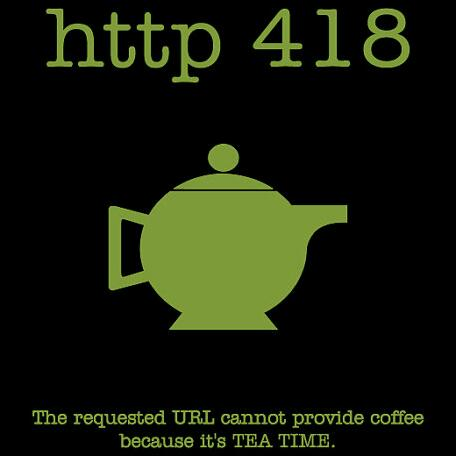
\includegraphics[scale=0.3]{../teamPic.jpg}					
			}								
		}
	\end{titlepage}
	\newpage
	\section{The Team}
	\subsection{LC Meyers}
	\begin{figure}[h]
		\centering
		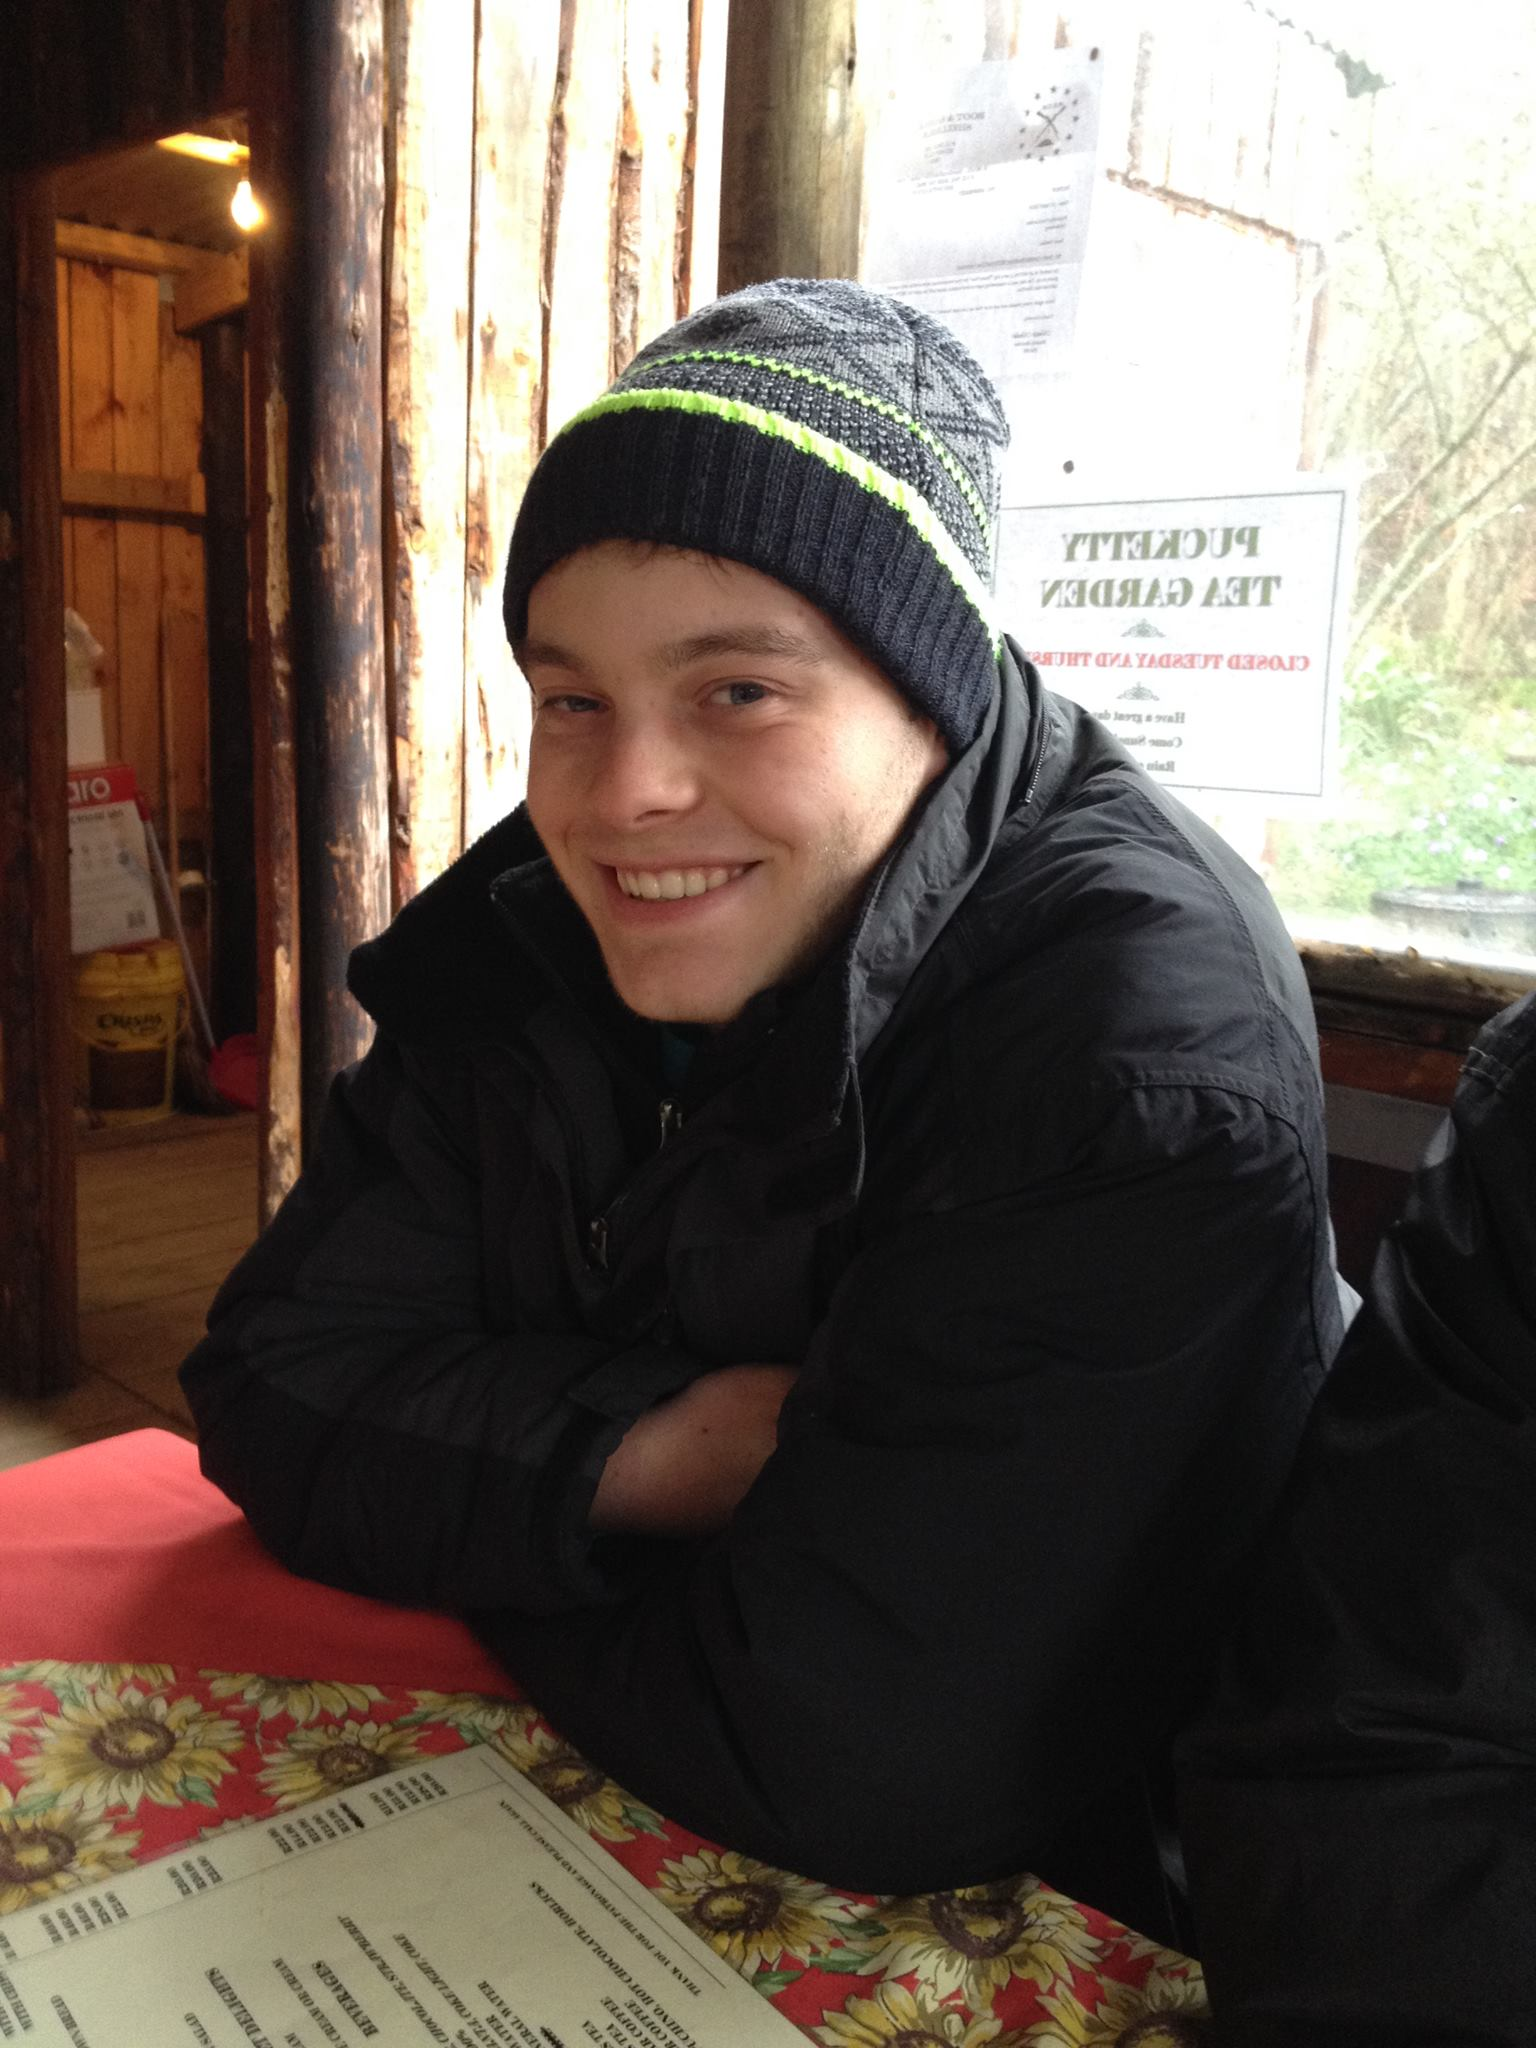
\includegraphics[height=0.3\textheight]{../charl.jpg}
	\end{figure}
	\begin{itemize}
		\item \textbf{Full name:} Lodewyk Charles Meyers
		\item \textbf{My interests:}
			\subitem Gaming
			\subitem Computers
			\subitem Music
			\subitem User experience design
			\subitem Website design
			\subitem Anything new related to technology
		\item \textbf{My technical skills:}
			\subitem Web development skills
			\subitem Database design
			\subitem Java
			\subitem C\#
		\item \textbf{Past experience that might help:}
			\subitem I collaborated on a website for a school as part of a project.			
		\item \textbf{Non-technical strenghts:}
			\subitem I have a high amount of patience
			\subitem Hardworking
			\subitem Eager to learn new things
			\subitem Enjoy trying to solve complex problems
		\item \textbf{What makes me want to do this project?} I love web development and will enjoy this project a lot. I still want to learn how to use C\# for a web server and web based development and this project will be the perfect opportunity for me to learn C\# web based development.
	\end{itemize}
	
	\subsection{EF Bode}
	\begin{figure}[h]
		\centering
		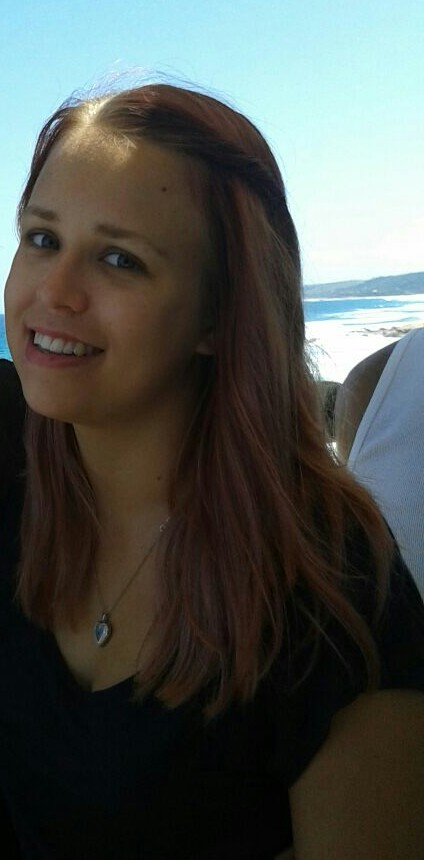
\includegraphics[height=0.3\textheight]{../Liz.jpg}
	\end{figure}
	\begin{itemize}
		\item \textbf{Full Name:} Elizabeth Fae Bode
		\item \textbf{My Interests:}
		\subitem Puzzle Games (eg. Sudoku)
		\subitem Computers
		\subitem Art
		\subitem Music
		\subitem User experience design
		\subitem Website design
		\subitem Gardening
		\subitem Reading books
		
		\item \textbf{My Technical Skills:}
		\subitem Web development skills
		\subitem Database design
		\subitem Java
		\subitem C\#
		\subitem C++
		\subitem Good at writing
		
		\item \textbf{Past Experience that Might Help:} \newline
		I have experience in both C\# and web-based development, however, I do not have a lot of experience in web-based C\# development. I have a willingness to learn though and thoroughly enjoy web-development so I think on this factor alone, that I would be a good candidate for the development of this application. I also have experience in both accounting and mathematics and I enjoyed them both quite a lot at school and again at university.
		
		\item \textbf{Non-technical Strengths:}
		\subitem Good at decision-making
		\subitem Good at problem-solving
		\subitem Hardworking
		\subitem Organised
		\subitem Responsible
		\subitem Eager to learn new things
		\subitem Perfectionist
		
		\item \textbf{What makes me want to do this project?} \newline
		As I mentioned, I have experience in both accounting and mathematics, both of which I am passion about. This passion is made me interested in this project as I love applications that integrate complex calculations with simple but very useful functionality. I enjoy developing in C\# and I enjoy developing functional applications that provide immense value to companies. All these things together, make me really interested in implementing this project.
	\end{itemize}

		\subsection{C Saaiman}
	\begin{figure}[h]
		\centering
		
\includegraphics[height=0.3\textheight]{Saaiman.jpg}
	\end{figure}
    
    \begin{itemize}
    \item \textbf{Full Name:} Christiaan Saaiman
    \item \textbf{My interests:}
    	\subitem Reading books
        \subitem Piano playing
        \subitem Gaming
        \subitem Coding
        \subitem Web Design
        \subitem User Experience Design
        \subitem Cooking and Baking
		\subitem Anime
        \subitem Languages
        	\subsubitem German
            \subsubitem Italian
            \subsubitem Japanese
        \subitem Artificial Intelligence
        \subitem Phones, Computer Hardware and Next-Gen Consoles

	\item \textbf{Technical Skills:}
    	\subitem Web Development Skills
        \subitem Java
        \subitem C++
        
	\item \textbf{Past experience:}
    	\subitem 6 Months intensive Java Training Course
        \subitem 6 Month Internship at Accenture
        	\subsubitem Intense Oracle Systems Training
            \subsubitem Leadership Training and meetings with the MD of Technology
            \subsubitem pitching an idea a colleague and I had.
            \subsubitem Tiger Brands' System upgrade from Oracle Database 11g to 12c
        \subitem Android App development using PhoneGap
    \item \textbf{Non-technical Strengths:}
    	\subitem Excellent Leader, not  afraid of conflict
        \subitem Excellent communicator
        \subitem Curious and eager to take on challenges
        \subitem Problem solver
        \subitem Dedicated and hardworking
        \subitem Creative and spontaneous
        
   \item \textbf{Reason for Project Tender:} \newline
   The project proposal peaked my interest in several ways. Firstly I was curious to extend my		      knowledge with regards to the subtropical farming that is present in South Africa and how it plays    its role as a significant forex earner in our country. Secondly I was delighted to see that there      is a need for an application, as I wish to further extend and broaden my knowledge in the field of    Mobile Development. This project I believe I will tackle with enthusiasm and grit. Lastly I was        also intrigued by the thought of helping farmers with an app to help them better their yield. I      want to know more of how this could be further extended to help not only farmers, but other          business owners as well.
       
	\end{itemize}
	
	\section{Project excecution}
	\begin{itemize}
		\item \textbf{Development Methodology} \newline \newline
		We plan to follow the Agile development methodology as it involves regular communication with the client to ensure the project results in exactly what they want. It also has a focus on the people system and their interactions with it which we believe is way more important than focusing on the processes and tools of the system. We strive to maintain a continues attention to designing the system well and ensuring that all the technical aspects are coherent with the requirements. All of which makes the Agile development methodology perfect for our vision for your project.
		
		\item \textbf{Progress Communication Plan} \newline \newline
		We plan on meeting up with you as the client on a regular basis, either face-to-face or via Skype, whichever is more convenient for you at the time, in order to keep you updated regarding the status of the project and to clarify requirements. We are also willing to communicate either via WhatsApp or email, whichever you prefer, in order to discuss the project and the progress of it, if face-to-face meetings are unable to take place for whatever reasons.

		\item \textbf{Technologies we will use for the project:}
		\begin{itemize}
			\item For the front end we will use Bootstrap framework along with JQuery to handle AJAX requests to the server. Bootstrap makes making responsive websites very easy, thus the choice in Bootstrap.
			\item For the backend we will use C\# for the RESTful web server to serve the results of calculations to the client. If needed we can also use C\# for the front end of the system.	
		\end{itemize}
	\end{itemize}
\end{document}